% $Id:background.tex  $
% !TEX root = main.tex

\chapter{Background}
\section{Reinforcement Learning}
Reinforcement learning problem can be considered as training an agent to interact with an environment governed by a Markov Decision Process (MDP). A MDP is a mathematical framework used to model decision-making in situations where outcomes are partly random and partly under the control of a decision-maker. The agent would start in an initial state, for each interaction with MDP, the agent can take an action guided by a policy which leads into a new state and assigning to the agent a reward for the step it just took and an observation of the new state it just got in. This agent then, accumulates time-discounted rewards along with its interactions with the MDP. A set of subsequent interactions is known as a transition or episode. The RL problem consist of maximizing the time-discounted rewards along time\cite{Sutton2018}.

\begin{itemize}
    \item $S$ is a finite set of states representing the possible configurations of the system.
    \item $A$ is a finite set of actions available to the decision-maker.
    \item $P: S \times A \times S \rightarrow [0, 1]$ is the state transition probability function, where $P(s' | s, a)$ denotes the probability of transitioning from state $s$ to state $s'$ after taking action $a$.
    \item $R: S \times A \rightarrow \mathbb{R}$ is the reward function, which provides the immediate reward received after transitioning from state $s$ to state $s'$ due to action $a$.
    \item $\gamma \in [0, 1]$ is the discount factor, which determines the present value of future rewards.
\end{itemize}

The objective in an MDP is to find a policy $\pi: S \rightarrow A$ that maximizes the expected cumulative reward over time. This optimal policy guides the decision-maker's actions at each state to achieve the best possible outcome\cite{markovian_desicion_process_book}.

A visual representation of an MDP is provided in Figure \ref{fig:MDP Diagram}, illustrating the interaction between states, actions, rewards, and transitions.

\begin{figure}[ht]
    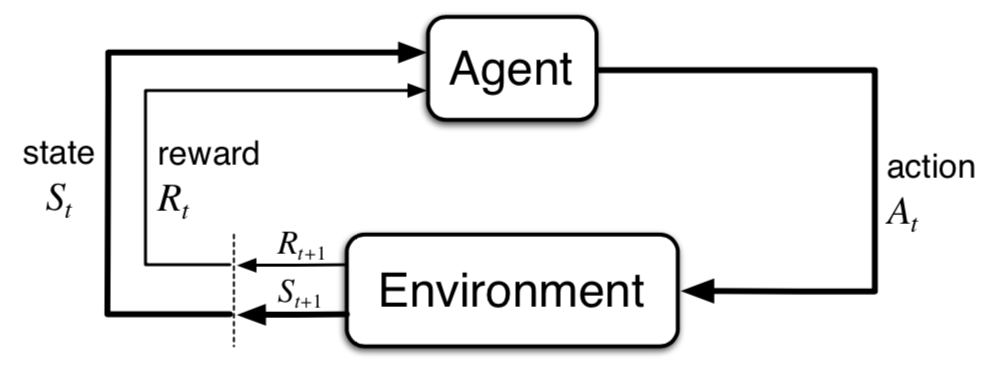
\includegraphics[width=\linewidth]{./figures/Agent-Environment.png}
    \centering
    \caption[MDP]{Markov decision process. Took from: \cite{Sutton2018}}
    \label{fig:MDP Diagram}
\end{figure}

\subsection*{Policy}
A \emph{policy} is a mapping from a state to an action.

\begin{equation*}
    \pi_t(s|a)
    \label{eq: policy}
\end{equation*}

That is the probability of select an action $A_t = a$ if $S_t = s$.

\subsection*{Reward and Return}
The reward function $R$ plays a crucial role in reinforcement learning, as it is determined by the current state of the environment, the action just taken, and the resulting next state.

\begin{equation*}
    r_t=R(s_t, a_t, s_{t+1})
\end{equation*}

Is frequently simplified to to just a dependence on the current state $r_t=R(s_t)$ or state action pair $r_t=R(s_t, a_t)$.

The agent's objective is to maximize a certain measure of cumulative reward over a trajectory, the return, but this can take several forms. The notation of these scenarios is $R(\tau)$, and it will either be clear from the context which specific case is being referred to, or it won't be significant, as the same equations will apply in all cases.

The total \emph{reward} is expressed as:

\begin{equation*}
    G_t = \sum_{k = 0}^H \gamma^kr_{t + k + 1}
    \label{eq: total_reward}
\end{equation*}

Where $\gamma$ is the \emph{discount factor} and $H$ is the \emph{horizon}, that can be infinite.

\subsection*{Value functions}

In a MDP the value function quantifies the expected cumulative reward an agent can achieve from a given state (or state-action pair). It helps evaluate how good it is for the agent to be in a particular state, or to take a certain action from that state, with the goal of maximizing long-term rewards. There are two common types of value functions, The \emph{State Value function (V)} and the \emph{Action-Value function (Q)}.
Tha \emph{State Value function} denoted as $V_(s)$ represents the expected cumulative reward when starting from state $s$ and following a given policy $\pi$ thereafter:

\begin{equation}
    V^\pi(s) = \mathbb{E}_\pi \left[ \sum_{t=0}^{\infty} \gamma^t r_{t+1} \mid s_t = s \right]
    \label{eq: value_suboptimal}
\end{equation}

The \emph{Action-Value function} also known as the Q-function, denoted as $Q(s,a)$ represents the expected cumulative reward when starting from state $s$, taking an action $a$, and then following a given policy $\pi$:

\begin{equation}
    Q^\pi(s, a) = \mathbb{E}_\pi \left[ \sum_{t=0}^{\infty} \gamma^t r_{t+1} \mid s_t = s, a_t = a \right]
    \label{eq: q_func_suboptimal}
\end{equation}

Clearly, using this new notation we can redefine $V^*$, equation \ref{eq: value_suboptimal}, using $q^*(s,a)$, equation \ref{eq: q_func_suboptimal}:

\begin{equation}
    V_*(s) = \max\limits_{a \in A(s)} q_{\pi*}(s,a)
\end{equation}

Intuitively, the above equation express the fact that the value of a state under the optimal policy \textbf{must be equal} to the expected return from the best action from that state.

Value functions helps the agent to make decisions by estimating the long-term benefits of being in certain states or taking specific actions.

\section{Bellman Equation}
The fundamental idea of the Bellman equations is that the value of the starting state is the expected reward from being in that state, combined with the value of the next state you reach.The Bellman Equation simplifies a complex problem by breaking it into smaller, more manageable steps. It helps determine the optimal decision-making strategy when outcomes depend on a sequence of actions. Bellman equations are expressed as:

\begin{equation*}
    V^\pi(s) = \underset{a \thicksim \pi}{\mathbb{E}} \left[ r(s,a) + \gamma V^\pi (s^{\prime}) \right]
\end{equation*}

\begin{equation}
    Q^\pi(s,a) =\underset{s^{\prime}\thicksim P}{\mathbb{E}} \left[ r(s,a) + \gamma \underset{a^{\prime}\thicksim \pi}{\mathbb{E}}\left[Q^{\pi}(s^{\prime},a^{\prime})\right]\right]
    \label{eq: q-value-bellman-equation}
\end{equation}

\section{Deep reinforcement learning algorithms}
This document focuses on Deep reinforcement learning, which uses neural networks to model traditional reinforcement learning algorithms and focuses on \emph{Temporal-Difference Learning} or TD which is an alternative to methods. Temporal difference learning focuses to solve RL problem so that both value function and policy can get improved simultaneously\cite{Sutton2018}. Some examples of \emph{Temporal difference} algorithms are SARSA\cite{SARSA}. Actor Critic\cite{SAC}. Q-learning algorithms for discrete state-action spaces that use deep neural networks exists as well such as Deep Q-Learning\cite{deep_q_learning}.

TD-learning methods, like Q-learning, focus on estimating state-action value functions. In contrast, Policy Gradient methods aim at directly optimizing a parameterized policy. Traditional policy gradient approaches include algorithms such as REINFORCE\cite{reinforce_algorithm}. In recent years, there has been a convergence of TD-learning and policy gradient methods, largely due to advancements in deep neural networks. Notable algorithms in this area include Trust Region Policy Optimization (TRPO)\cite{TRPO}, Proximal Policy Optimization (PPO)\cite{ppo}, Deep Deterministic Policy Gradient (DDPG)\cite{ddpg} and Twin Delayed DDPG\cite{TD3}.

\section{Deep Q Learning and Deep Deterministic Policy Gradient}
In practice, the basic approach of iterating over the Bellman equation of the Q-values\ref{eq: q-value-bellman-equation}, since the action-value function is estimated independently for each sequence, with no generalization. Created by $DeepMind$, Deep Q Learning (DQL)\cite{deep_q_learning}, substitutes the $Q$ function with a deep neural network called \emph{Q-network}. This \emph{Q-network} is going to be updated by minimizing a sequence of a loss function defined by:

\begin{equation}
    L_i(\theta_i) = \mathbb{E}_{(s, a, r, s') \sim U(D)}\begin{bmatrix}
        ( \underbrace{r + \gamma \max\limits_a Q(s',a'; \theta_{i-1})}_\text{target} - \underbrace{Q(s,a;\theta_i)}_\text{prediction})^2
    \end{bmatrix}
\end{equation}
Where $\theta$ are the weights of the network and $U(D)$ is the experience replay history.

DQL algorithm also keep track of some observation in a $memory$ in order to use them to train the network, this is used to avoid the time correlation and make the samples to be more independently and identically distributed. the full algorithm can be found in algorithm \ref{al: dqn}.

\hfil\break
\begin{algorithm}[H]
    \caption{Deep Q Learning algorithm}
    Initialize replay memory $D$ with capacity $N$\\
    Initialize $Q(s,a)$ arbitrarily \\
    \ForEach{episode $\in$ episodes}{
        \While{$s$ is not terminal} {
            With probability $\epsilon$ select a random action $a \in A(s)$ \\
            otherwise select $a = \max_a Q(s, a; \theta)$ \\
            Take action $a$, observer $r, s'$ \\
            Store transition $(s, a, r, s')$ in $D$ \\
            Sample random mini batch of transitions $(s_j, a_j, r_j, s'_j)$ from $D$ \\
            $\text{Set } y_j \leftarrow
                \begin{cases}
                    r_j                                         & \text{for terminal } s_j'     \\
                    r_j + \gamma \max\limits_a Q(s',a'; \theta) & \text{for non-terminal } s'_j
                \end{cases}$ \\
            Perform gradient descent step on $(y_j - Q(s_j, a_j;\Theta))^2 $ \\
            $s \leftarrow s'$
        }
    }
    \label{al: dqn}
\end{algorithm}

\hfil\break
which mins that the  actor is updated by following the applying the chain rule to the expected return from the start distribution $J$ with respect to the actor parameters.

Deep Q learning has a downside, it is not suitable for continuous action spaces. When the set of possible actions is finite and discrete, computing the maximum presents no difficulty. One can simply evaluate the Q-values for each action individually and determine the highest value. This also immediately identifies the action that maximizes the Q-value. However, when the action space is continuous, exhaustive evaluation becomes impractical, and solving the associated optimization problem is considerably complex. Employing a conventional optimization algorithm to compute $\max_a Q^*(s,a)$ would result in an extremely costly subroutine. Given that this computation would be required each time the agent selects an action within the environment, such an approach is infeasible. To address this limitation, Deep Deterministic Policy Gradient (DDPG) was introduced. DDPG is an off-policy algorithm that uses a deterministic policy and a Q-function to learn the optimal policy in continuous action spaces. It also employs a replay buffer to store experiences and uses a target network to stabilize learning.

The Deterministic Policy Gradient (DPG)\cite{DPG} algorithm employs a parameterized actor function $\mu(s | \theta_\mu)$ that defines the current policy by deterministically associating states with specific actions. The critic function $Q(s, a)$ is learned through the Bellman equation, similar to Q-learning. The actor's parameters are updated by applying the chain rule to the expected return $J$ from the initial state distribution, ensuring an optimized policy adjustment. 

Similar to Deep Q-Networks (DQN), a replay buffer is utilized to mitigate the challenge of avoiding the states to be time correlated. The replay buffer, denoted as $R$, is a finite-sized cache that stores transitions sampled from the environment following an exploration policy. Each transition, represented as the tuple $(s_t, a_t, r_t, s_{t+1})$, is added to the buffer. When the buffer reaches capacity, the oldest samples are removed to make space for new data. At every time step, the actor and critic are refined by uniformly sampling a mini batch from the buffer. Since Deep Deterministic Policy Gradient (DDPG) operates as an off-policy algorithm, the replay buffer can be substantially large, enabling the algorithm to leverage learning across a diverse set of uncorrelated transitions. DDPG works as an actor critic algorithm, where the actor is responsible for selecting actions based on the current policy, while the critic evaluates the actions taken by the actor. The critic is trained to minimize the mean squared error between the predicted Q-values and the target Q-values, which are computed using the Bellman equation.

Consider a neural network, $Q_{\phi}(s,a)$, as a policy approximator, where $\phi$ represents its parameters. Suppose we have gathered a dataset $\mathcal{D}$ comprising transitions $(s,a,r,s',d)$, with $d$ indicating whether the state $s'$ is terminal. One can define the mean squared Bellman error function, which provides an estimate of how well $Q_{\phi}$ adheres to the Bellman equation\ref{eq: q-value-bellman-equation}.

\begin{equation*}
    L(\phi, \mathcal{D}) = \mathbb{E}_{(s,a,r,s',d)\sim\mathcal{D}}\left[\left(Q_{\phi}(s,a) - y(r,s',d)\right)^2\right]
\end{equation*}

where $y(r,s',d)$ is the target value, defined as:
\begin{equation*}
    y(r,s',d) = r + \gamma(1-d)\max_{a'} Q_{\phi}(s',a')
\end{equation*}

DDPG algorithm also applies a target network to stabilize the learning process. The target networks are copies of the actor and critic networks, which are updated slowly to ensure stability during training. The target networks are updated using a soft update mechanism, where the target parameters are updated as follows:

\begin{equation*}
    \theta_{\text{targ}} \leftarrow \tau\theta_{\text{targ}} + (1-\tau)\theta
\end{equation*}

The actor or so called \emph{policy} is updated by following the applying the chain rule to the expected return from the start distribution $J$ with respect to the actor parameters. The objective is to learn a deterministic policy, $ \mu_{\theta}(s) $, that selects the action maximizing $ Q_{\phi}(s,a) $. Given that the action space is continuous and assuming that the Q-function is differentiable with respect to the action, we can apply gradient ascent—focusing solely on policy parameters—to find the optimal solution.

\begin{equation*}
    \max_{\theta} \mathbb{E}_{s\thicksim\mu_0}\left[Q_{\phi}(s,\mu_{\theta}(s))\right]
\end{equation*}

The DDPG algorithm is summarized in Algorithm \ref{al: ddpg}.

\begin{algorithm}[!ht]
    \caption{Deep Deterministic Policy Gradient Algorithm}
    \label{al: ddpg}
    Input: initial policy parameters $\theta$, Q-function parameters $\phi$, empty replay buffer $\mathcal{D}$\;
    Set target parameters equal to main parameters $\theta_{\text{targ}} \leftarrow \theta$, $\phi_{\text{targ}} \leftarrow \phi$\;
    \Repeat{convergence}{
        Observe state $s$ and select action $a = \text{clip}(\mu_\theta(s) + \epsilon, a_{\text{Low}}, a_{\text{High}})$, where $\epsilon \sim \mathcal{N}$\;
        Execute $a$ in the environment\;
        Observe next state $s'$, reward $r$, and done signal $d$ to indicate whether $s'$ is terminal\;
        Store $(s,a,r,s',d)$ in replay buffer $\mathcal{D}$\;
        If it's terminal, reset the environment\;
        \If{It's time to update}{
            \For{however many updates}{
                Rnadomly sample a batch of transitions, $B = \{(s,a,r,s',d)\}$ from $\mathcal{D}$\;
                Compute target:
                \hspace{3.5cm}$y(r,s',d) = r + \gamma(1-d)\max_{a'} Q_{\phi_{\text{targ}}}(s',a')$\;
                Update Q-function by one step of gradient descent using\;
                \hspace{3.5cm}$\nabla_{\phi}\frac{1}{|B|}\sum_{(s,a,r,s',d)\in B}(Q_{\phi}(s,a) - y(r,s',d))^2$\;
                Update policy by one step of gradient ascent using:
                \hspace{3.5cm}$\nabla_\theta\frac{1}{|B|}\sum_{s\in B}Q_{\phi}(s,\mu_\theta(s))$\;
                Update target networks with:
                \hspace{3.5cm}$\phi_{\text{targ}} \leftarrow \rho\phi_{\text{targ}} + (1-\rho)\phi$\;
                \hspace{3.5cm}$\theta_{\text{targ}} \leftarrow \rho\theta_{\text{targ}} + (1-\rho)\theta$\;
            }
        } 
    }
\end{algorithm}
\clearpage

\section{Twin Delayed DDPG (TD3)}
Deep Deterministic Policy Gradient (DDPG) can sometimes achieve strong performance; however, it tends to be sensitive to hyperparameter and other tuning aspects. A common failure mode arises when the learned Q-function significantly overestimates Q-values, causing the policy to exploit these inaccuracies, ultimately leading to instability. Twin Delayed Deep Deterministic Policy Gradient mitigates this issue through three fundamental techniques:

\textbf{Clipped Double-Q Learning:} TD3 employs two Q-functions instead of one and utilizes the lower Q-value for target calculation in the Bellman error loss functions, reducing overestimation.

\textbf{Delayed Policy Updates:} The frequency of policy updates in TD3 is reduced compared to Q-function updates, following the recommendation of one policy update for every two Q-function updates.

\textbf{Target Policy Smoothing:} Noise is introduced to the target action in TD3, ensuring smoother Q-value estimates and preventing the policy from exploiting discrepancies in the learned Q-function.

Collectively, these modifications lead to significant improvements in stability and performance compared to baseline DDPG\cite{TD3}.

TD3 optimizes two Q-functions, $Q_{\phi_1}$ and $Q_{\phi_2}$, by minimizing the mean squared Bellman error, following a process similar to the single Q-function learning in DDPG. To illustrate the mechanics of TD3 and its distinctions from standard DDPG, the explanation begins at the core of the loss function and expands outward.

Actions are taken directly from the policy $\mu_\theta$ plus a clipped noise and this actions is then clipped to not exceed the action space limits. So the action are calculated as:

\begin{equation*}
    a'(s') = \text{clip} \left(\mu_{\text{targ}}(s') + \text{clip}(\epsilon, -c, c), a_{Low}, a_{High}\right), \quad \epsilon \sim \mathcal{N}(0, \sigma)
\end{equation*}

Both Q-functions use a single target, calculated using whichever of the two Q-functions gives a smaller target value.

\begin{equation*}
    L(\phi_1, \mathcal{D}) = \mathbb{E}_{(s,a,r,s',d)\sim\mathcal{D}}\left[\left(Q_{\phi_1}(s,a) - y(r,s',d)\right)^2\right],
\end{equation*}

\begin{equation*}
    L(\phi_2, \mathcal{D}) = \mathbb{E}_{(s,a,r,s',d)\sim\mathcal{D}}\left[\left(Q_{\phi_2}(s,a) - y(r,s',d)\right)^2\right].
\end{equation*}

Selecting the lower Q-value as the target and adjusting predictions accordingly helps mitigate the risk of overestimation in the Q-function, the policy is then learned just by maximizing $Q_{\phi_1}$.

\begin{equation*}
    \max_{\theta} \mathbb{E}_{(s,a,r,s',d)\sim\mathcal{D}}\left[Q_{\phi_1}(s,\mu_\theta(s))\right]
\end{equation*}

TD3 is similar to DDPG, but it uses two Q-functions and a single target policy. The target policy is updated less frequently than the Q-functions, and noise is added to the target action to improve stability. The TD3 algorithm is summarized in Algorithm \ref{al: td3}.

TD3 employs an off-policy approach to train a deterministic policy. Since deterministic policies limit exploratory behavior when following an on-policy strategy, the agent might initially fail to sample a sufficiently diverse set of actions, reducing its ability to learn effectively. To enhance exploration during training, noise is introduced into the actions, typically using uncorrelated mean-zero Gaussian noise. Adjusting the noise scale over time can help generate higher-quality training data, though in our implementation, the noise scale remains constant throughout the training process.

\begin{algorithm}[ht]
\caption{Twin Delayed DDPG}
    \label{al: td3}
    Input: initial policy parameters $\theta$, Q-function parameters $\phi_1$, $\phi_2$, empty replay buffer $\mathcal{D}$\;
    Set target parameters equal to main parameters $\theta_{\text{targ}} \leftarrow \theta$, $\phi_{\text{targ},1} \leftarrow \phi_1$, $\phi_{\text{targ},2} \leftarrow \phi_2$\;
    \Repeat{convergence}{
        Observe state $s$ and select action $a = \text{clip}(\mu_\theta(s) + \epsilon, a_{\text{Low}}, a_{\text{High}})$, where $\epsilon \sim \mathcal{N}$\;
        Execute $a$ in the environment\;
        Observe next state $s'$, reward $r$, and done signal $d$ to indicate whether $s'$ is terminal\;
        Store $(s,a,r,s',d)$ in replay buffer $\mathcal{D}$\;
        \If{it's time to update}{
            \For{$j$ in range(however many updates)}{
                Randomly sample a batch of transitions, $B = \{(s,a,r,s',d)\}$ from $\mathcal{D}$\;
                Compute target actions\;
                $a'(s') = \text{clip}(\mu_{\text{targ}}(s') + \text{clip}(\epsilon, -c, c), a_{\text{Low}}, a_{\text{High}})$, $\epsilon \sim \mathcal{N}(0,\sigma)$\;
                Compute targets\;
                $y(r,s',d) = r + \gamma(1-d)\min_{i=1,2} Q_{\phi_{\text{targ},i}}(s',a'(s'))$\;
                Update Q-functions by one step of gradient descent using\;
                $\nabla_{\phi_i}\frac{1}{|B|}\sum_{(s,a,r,s',d)\in B}(Q_{\phi_i}(s,a) - y(r,s',d))^2$ for $i=1,2$\;
                \If{$j$ mod policy\_delay $= 0$}{
                    Update policy by one step of gradient ascent using\;
                    $\nabla_\theta\frac{1}{|B|}\sum_{s\in B}Q_{\phi_1}(s,\mu_\theta(s))$\;
                    Update target networks with\;
                    $\phi_{\text{targ},i} \leftarrow \rho\phi_{\text{targ},i} + (1-\rho)\phi_i$ for $i=1,2$\;
                    $\theta_{\text{targ}} \leftarrow \rho\theta_{\text{targ}} + (1-\rho)\theta$\;
                }
            }
        }
    }
\end{algorithm}
\clearpage

\section{CARLA: An Open-Source Urban Driving \\simulator}

\begin{figure}[ht]
    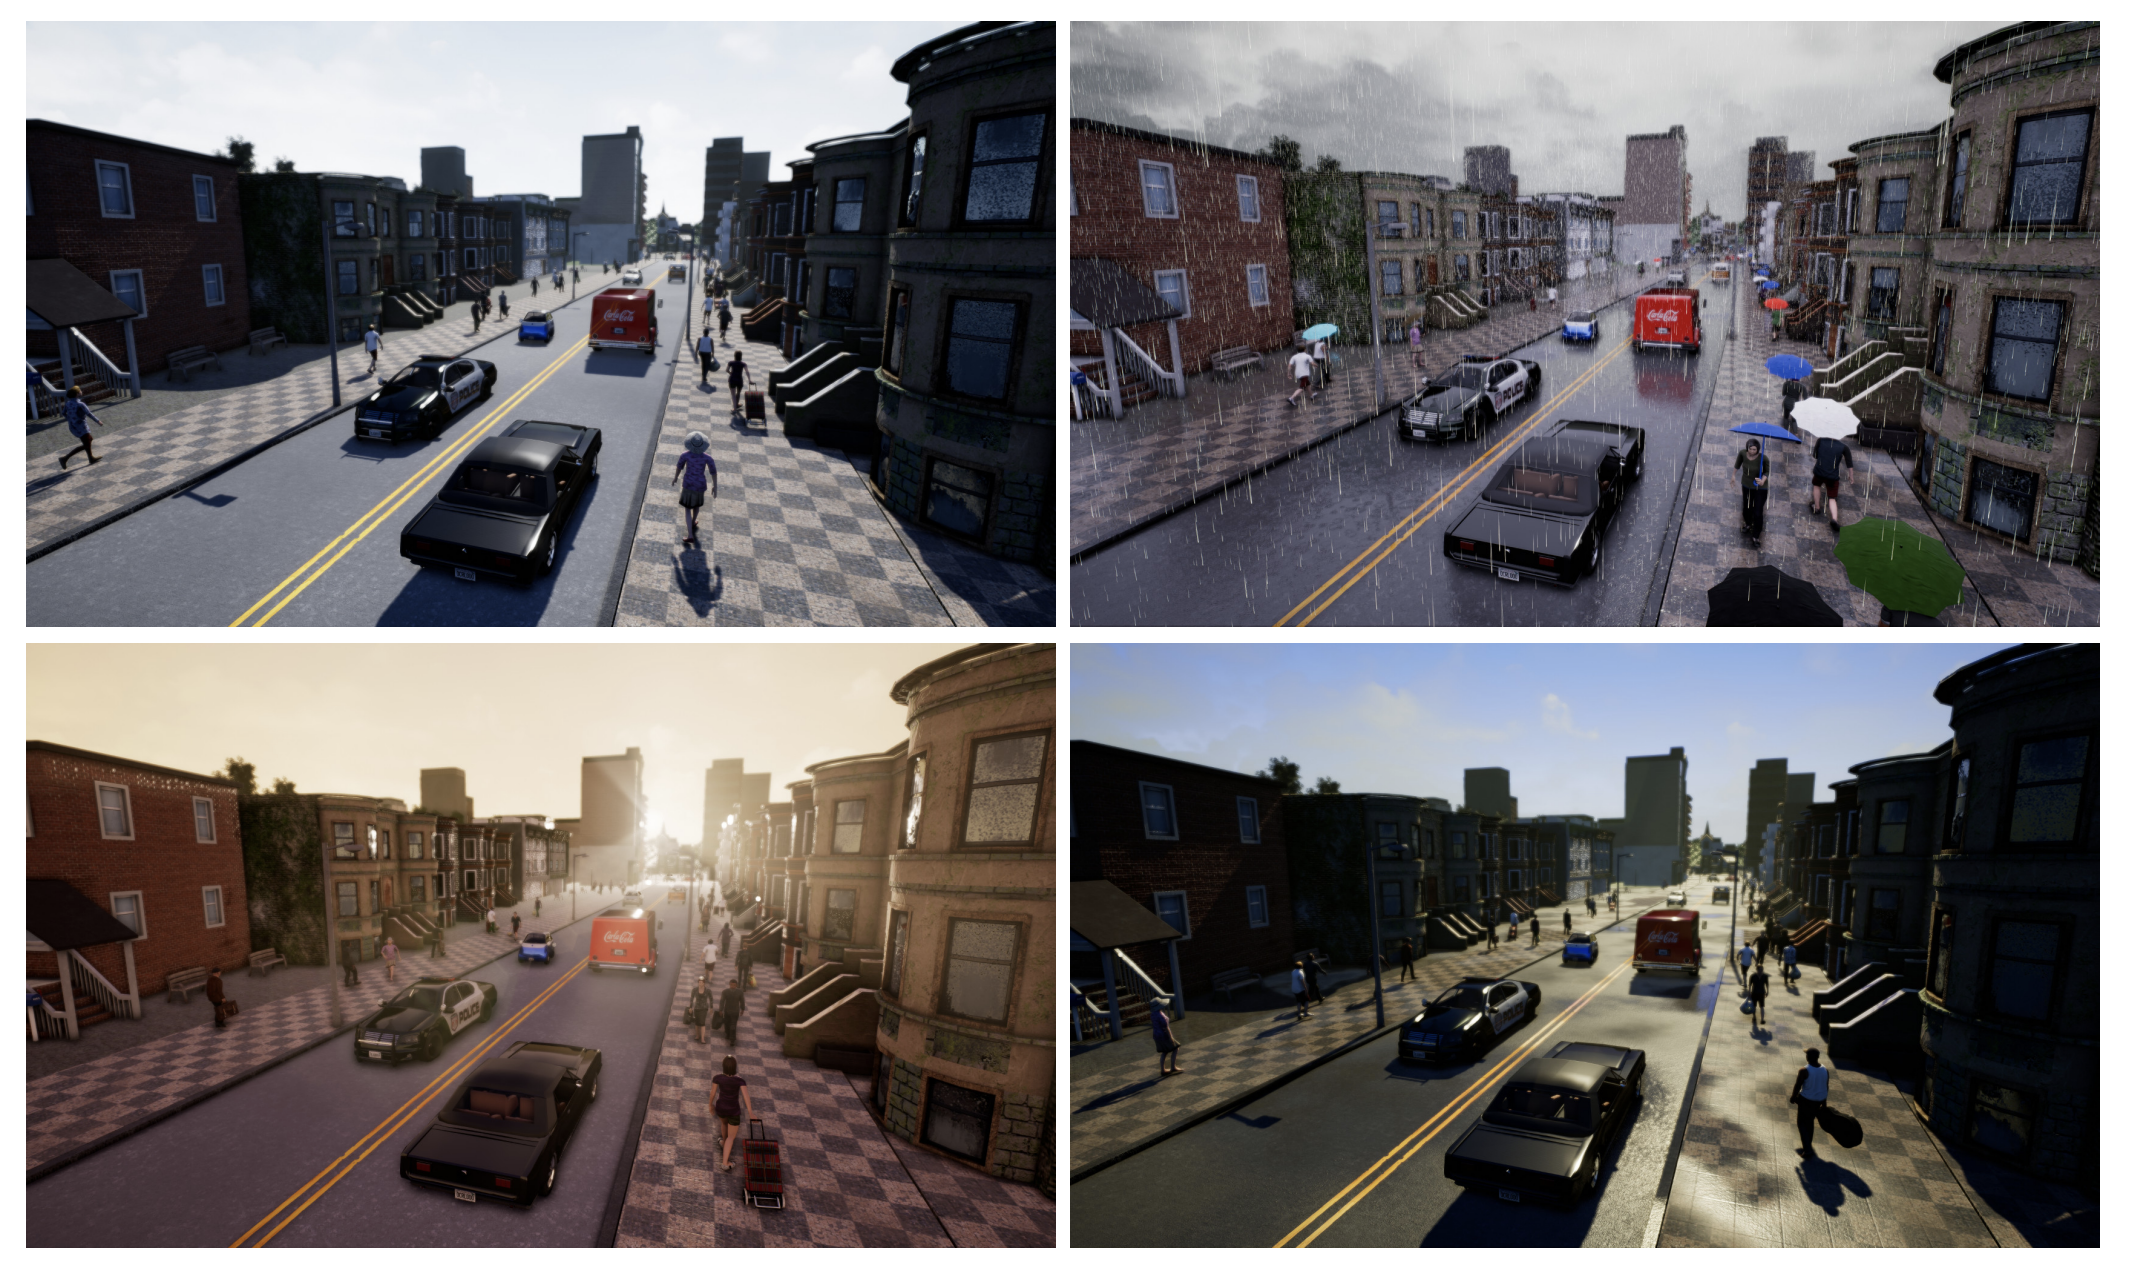
\includegraphics[width=\linewidth]{./figures/Carla-simulator.png}
    \centering
    \caption[CARLA Simulator]{CARLA Simulator benchmark}
    \label{fig:CARLA Simulaor}
\end{figure}

CARLA (Car Learning to Act) is an open source simulator specifically designed for autonomous driving research. It provides a high-fidelity environment for the development, training, and validation of autonomous driving systems.

CARLA is built on top of Unreal Engine 4, which allows for realistic rendering and physics simulation, providing a detailed and dynamic urban environment\cite{CARLA}.

The simulator supports a wide range of sensors, including cameras, LiDAR, RADAR, and GPS, which can be configured to emulate the sensor setups used in real autonomous vehicles. Additionally, CARLA offers flexible APIs that allow researchers to control various aspects of the environment, such as weather conditions, time of day, and traffic density, as well as to introduce various actors like vehicles and pedestrians into the simulation.

Pedestrians move through the town using a navigation map specific to each area, which assigns a cost to different locations. This cost system encourages pedestrians to follow sidewalks and designated crosswalks but does not restrict them from crossing streets elsewhere. As they roam the town, pedestrians interact with one another, attempting to avoid collisions and steering clear of vehicles. If a pedestrian is hit by a vehicle, they are removed from the simulation, and a new pedestrian is generated at a different location after a short delay.

One of CARLA's significant contributions is its extensive benchmark suite, which enables standardized evaluation of autonomous driving algorithms. This includes tasks such as perception, planning, and control. Moreover, CARLA facilitates the collection of large-scale, diverse datasets, which are essential for training machine learning models in autonomous driving. As shown in Figure \ref{fig:CARLA Simulaor} is represented the same town but with different weather conditions to simulate a dynamic environment.

\section{Robot Operating system}
ROS (Robot Operating System) is an open source framework for developing specialized robotics software. It consists of a series of libraries, conventions and tools to create a robust specialized work environment. It has a variety of features, the name operating system (OS) is due to the fact that it has functionalities such as hardware abstraction, message passing between processes, among others, similar to that of an OS as shown in figure \ref{fig: ros as a framework}. However, a more appropriate name would be meta operating system since ROS operates on an operating system such as Linux \cite{ros_web} One of its most important parts is the communication infrastructure. It offers an interface for transferring information in the form of messages; usually this communication between components is one of the first needs when creating any robot.

\begin{figure}[ht]
    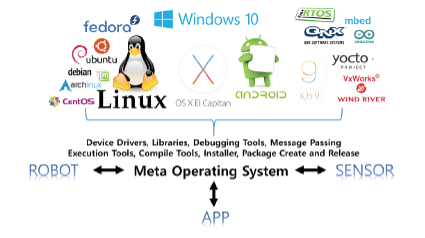
\includegraphics[width=0.6\textwidth]{./figures/ROS_FRAMEWORK.png}
    \centering
    \caption{Diagram of ROS as a meta operating system.}
    \label{fig: ros as a framework}
\end{figure}

Its basic operation is best explained as a graph architecture. In a simplified way, ROS allows you to create communication nodes, which are executable files with ROS commands inside a ROS package. These nodes communicate through topics. In turn, a topic can \emph{publish} messages for another topic to \emph{subscribe} to and vice versa. The ROS Master node will start with the first initialized node and will be in charge of managing the other nodes as shown in figure \ref{fig: ros nodes graph}.

\begin{figure}[ht]
    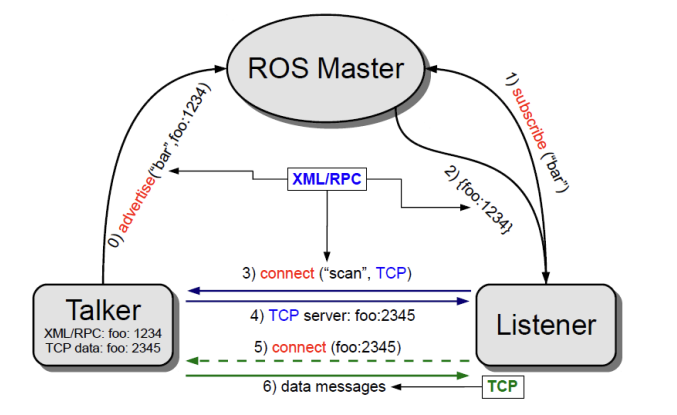
\includegraphics[width=0.5\textwidth]{./figures/ros_nodes.png}
    \centering
    \caption{Computational Graph of a ROS node.}
    \label{fig: ros nodes graph}
\end{figure}

Likewise, ROS has a package called \emph{gazebo\_ros} that allows its integration with Gazebo\cite{gazebo_url}, a simulator (shown in figure \ref{fig: gazebo showcase}) that is largely faithful to reality since it include in its software physics engines such as ODE\footnote{ODE physics simulator: \url{https://www.ode.org/}},Bullet\footnote{Bullet physics engine: \url{https://pybullet.org/wordpress}}, Simbody\footnote{Multibody physics API: \url{https://objectivesimtk.org/projects/simbody}} and DART\footnote{Dynamic Animation and Robotics Toolkit: \url{https://dartsim.github.io/}}. Because of this, the state of the simulated environment is highly accurate and always available, the covariances of the measurements when simulating sensors are amplified and Gaussian noise is added to the observed data, thus creating realistic scenarios that allow simulations to be carried out and data to be taken similar to that which would be obtained in the real environment.

\begin{figure}[ht]
    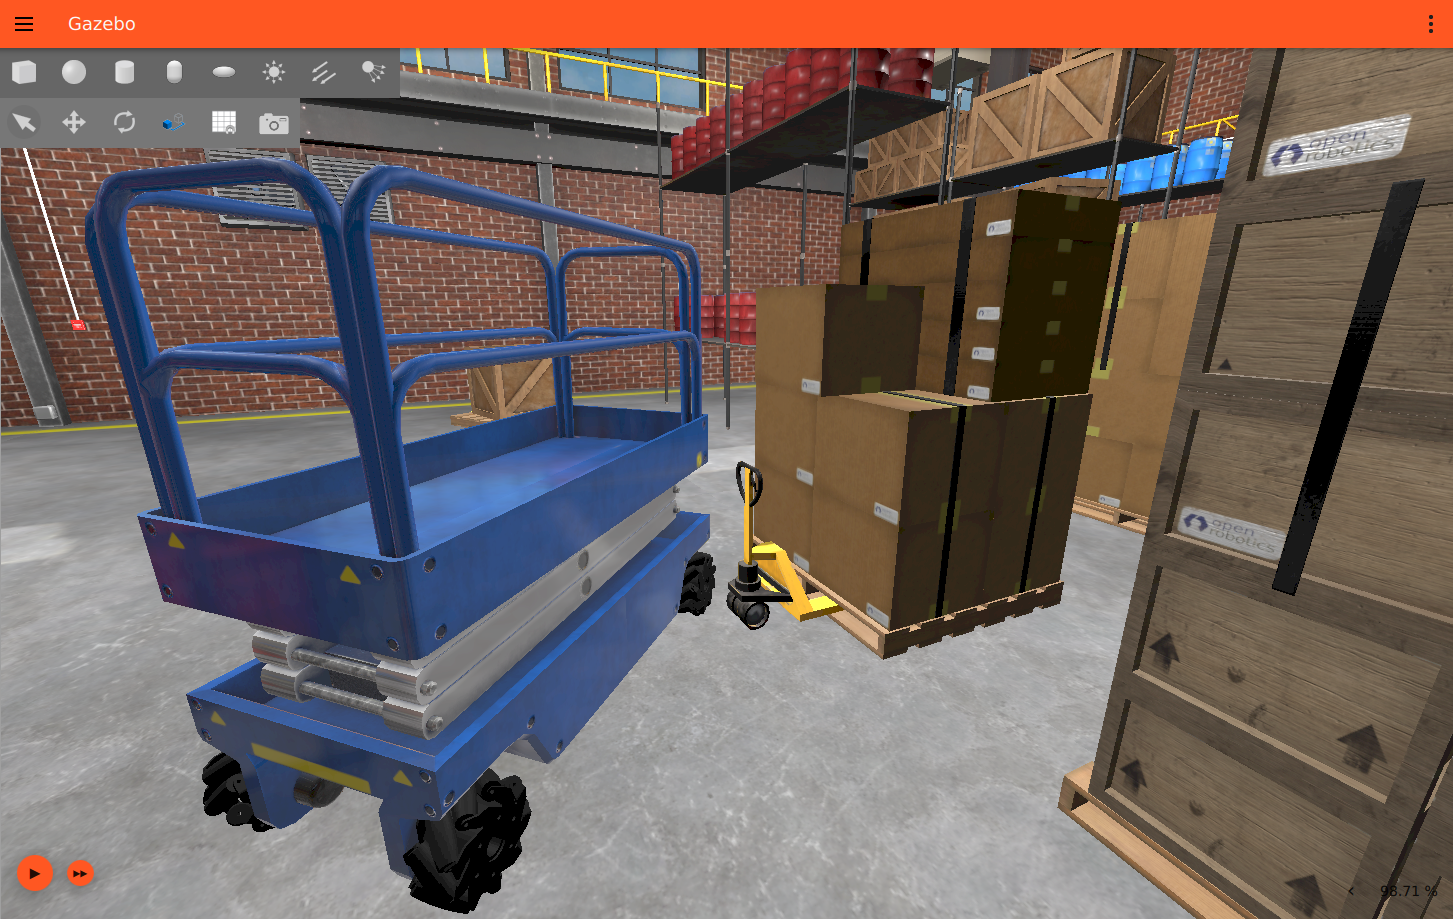
\includegraphics[width=0.7\textwidth]{./figures/gazebo_show.png}
    \centering
    \caption{Gazebo showcase: https://gazebosim.org/showcase.}
    \label{fig: gazebo showcase}
\end{figure}

\section{Transfer Learning}
There are several ways of transfer learning, numerous approaches have been explored to enhance reinforcement learning (RL) by incorporating different forms of supervision, often within distinct problem contexts. There are other techniques related to TL, examining their differences and connections may help to better define the relationship between TL and these approaches. \emph{Discriminator Actor-critic}\cite{imitation_learning} is one of them, they aim to train a policy by demonstrating the target actor an expert policy with few samples. This imitation could be more aggressive where the target actor is trained in a supervised manner with an expert policy\cite{imitation_learning_supervised}. Other form of transfer learning is \emph{Hierarchical Reinforcement Learning} (HRL) that has been proposed to focus on tasks where the actions space can be broken down into more simple action spaces to form a higher level macro of actions. Some algorithms of this kind could be Feudal learning\cite{feudal_rd}.

\emph{Multi-Agent Reinforcement Learning} or MARL is also another group of transfer learning algorithms, in this kind of framework, the MDP is considered with multiple actors interacting with the environment simultaneously and is focused to solve tasks that are not feasible to be learned by a single agent\cite{multi_agent_rl}.

TL tries to answer some questions like how the knowledge is stored or transferred, Whether or not all RL algorithms are compatible with TL, the significant of the difference between the source and the target domains or what is the goal to transfer learning. During a learned task, lets say \emph{Humanoid Standup}\footnote{Farama Humanoid standup: \url{https://gymnasium.farama.org/environments/mujoco/humanoid_standup/}}, the source and target domains $D$s can have differences such as the the state space, where one of them can have constraints that the other one does not have. The action space can also be different by changing the range of available forces that can be applied to the actuators. The reward function could be changed by encourage the agent do slight different behavior, or some actions can led into more penalty cost. Some differences can even reside in the trajectories where the source or target domain may allow shorter or larger total steps within the environment \cite{TL_survey}.

There are some other questions one can ask to try to find an answer to this question. How is the prior knowledge stored?. There's more than one answer to this question which some of them are going to be added in the following sections, but some of them one could think of in the context of reinforcement learning are to pass down the learned value function to the new task which is going to tell the agent which states and actions are good given a state, Or a learned policy which tells the agent which actions are potentially useful Or even a learned model such a physics of the environment or some learned rules by a prior agent that already learned the prior task \cite{TL_survey}. Lets first introduce formally TL in the context of reinforcement learning and then explore some of it's techniques.

Beyond transfer learning, numerous approaches have been explored to enhance reinforcement learning (RL) by incorporating different forms of supervision, often within distinct problem contexts. There are other techniques related to TL, examining their differences and connections may help to better define the relationship between TL and these approaches. \emph{Discriminator Actor-critic}\cite{imitation_learning} is one of them, they aim to train a policy by demonstrating the target actor an expert policy with few samples. This imitation could be more aggressive where the target actor is trained in a supervised manner with an expert policy\cite{imitation_learning_supervised}. Other form of transfer learning is \emph{Hierarchical Reinforcement Learning} (HRL) that has been proposed to focus on tasks where the actions space can be broken down into more simple action spaces to form a higher level macro of actions. Some algorithms of this kind could be Feudal learning\cite{feudal_rd}.
\emph{Multi-Agent Reinforcement Learning} or MARL is also another group of transfer learning algorithms, in this kind of framework, the MDP is considered with multiple actors interacting with the environment simultaneously and is focused to solve tasks that are not feasible to be learned by a single agent\cite{multi_agent_rl}.

As mention at the beginning of the section, some questions like how the knowledge is stored or transferred, Whether or not all RL algorithms are compatible with TL, the significant of the difference between the source and the target domains or what is the goal to transfer learning. During a learned task, lets say \emph{Humanoid Standup}\footnote{Farama Humanoid standup: \url{https://gymnasium.farama.org/environments/mujoco/humanoid_standup/}}, the source and target domains $D$s can have differences such as the the state space, where one of them can have constraints that the other one does not have. The action space can also be different by changing the range of available forces that can be applied to the actuators. The reward function could be changed by encourage the agent do slight different behavior, or some actions can led into more penalty cost. Some differences can even reside in the trajectories where the source or target domain may allow shorter or larger total steps within the environment \cite{TL_survey}.

The main challenge and question Transfer Learning tries to answer is wether a reinforcement learning algorithm could used prior knowledge from other tasks in the same way a humans do, i.e. Can an algorithm play better Montezuma's revenge\footnote{Montezuma's Revenge - Parker Brothers - Atari 2600 video game.} by letting it watch the movie. If prior tasks are solved, is it possible to acquire useful knowledge for solving new task?

Let $\mathcal{M}_s = \left\{\mathcal{M}_s|\mathcal{M}_s \in  \mathcal{M}_s\right\}$ be a set of source domains, which provides prior knowledge $\mathcal{D}_s$ that is accessible by the target domain $\mathcal{M}_t$, such that by leveraging the information from $\mathcal{D}_s$, the target agent learns better in the target domain $\mathcal{M}_t$, compared with not utilizing it.

In the context of Reinforcement Learning, given a set of source domains $\mathcal{M}_s$ and a target domain $\mathcal{M}_t$, Transfer Learning aims to learn an optimal policy $\pi^*$ for the target domain, by leveraging exterior information $\mathcal{D}_s$ from $\mathbf{\mathcal{M}_s}$ as well as interior information $\mathcal{D}_t$ from $\mathcal{M}_t$:

\begin{equation}
    \pi^* = \arg \max_{x} \mathbb{E}_{s\thicksim\mu^{t}_0,a\thicksim\pi}\left[Q^{\pi}_\mathcal{M}\left(s,a\right)\right]
\end{equation}

In TL is not a concern how much the source domain takes to learn but how the knowledge transfer accelerate the learning in the target domain.

One transfer learning technique is known as Reward Shaping (RS), which is a technique that leverages the exterior knowledge to reconstruct he reward distribution of the target domain tot guide the agent's policy learning. More specifically, in addition to the environment reward signals, RS learns a reward-shaping function $F: S \times  S \times A \to  \mathbb{R} $ to render auxiliary rewards, provided that the additional rewards contain external knowledge to guide the agent fo better action selection.

Intuitively, a reward shaped reward should be higher for actions that lead to more beneficial states.

Another technique is known as Domain adaptation, in reinforcement learning, domain adaptation refers to the process of transferring a learned policy from one domain, known as the source domain, to another, known as the target domain, where the two domains may differ in key aspects such as state representations, dynamics, or reward functions\cite{tsai2024proxymethodsdomainadaptation}. This concept is particularly relevant in scenarios where the agent is trained in a simulated environment, like CARLA, and then deployed in the real world, where environmental conditions and dynamics may vary.

The goal of domain adaptation is to ensure that a policy learned in the source domain remains effective in the target domain, despite these differences. By doing so, domain adaptation reduces the need for extensive training directly in the target domain, which may be costly or infeasible.

In this work, domain adaptation is critical, as the policies trained in the ROS simulator must be transferable to real-world scenarios. The key challenges in domain adaptation include:

\begin{itemize}
    \item \textbf{State Space Differences}: The state representation may vary between the source and target domains, such as different sensor inputs or noise characteristics. The agent needs to generalize its learned behavior across these discrepancies.

    \item \textbf{Dynamics Differences}: The underlying physical dynamics of the simulation and real world are rarely identical. For instance, the behavior of vehicles in the real world may differ due to friction, sensor latency, or other factors not perfectly captured in the simulation.

    \item \textbf{Reward Function Variability}: The reward structures in the source and target domains may differ. For example, while a policy may be optimized for smooth driving in simulation, real-world constraints such as safety or fuel efficiency may require adjustments.
\end{itemize}

Several strategies are employed to facilitate domain adaptation in RL:

\begin{itemize}
    \item \textbf{Domain Randomization}: This approach involves training the agent across multiple environments, where randomized simulation parameters define the goal positions and the ability to shift between left and right paradigms. By encountering a diverse range of configurations during training, the agent is better prepared to adapt and generalize to the target domain

    \item \textbf{Feature Alignment}: Techniques such as adversarial learning can be used to align the feature spaces of the source and target domains, ensuring that the agent's representations are robust to domain shifts.

\end{itemize}

Domain adaptation is an essential component of this work, as the goal is to ensure that policies developed within the CARLA simulation can generalize effectively to real-world driving environments.

\subsection*{Learning from demonstration}
Learning from demonstration is a technique to assist reinforcement learning using demonstrations either from human agents, an expert policy or even a sub-optimal policy. In our case we are going to use the previously trained agent to add an extra gradient when updating our actor and critic models. The idea is not to replace one agent with another, it is to somehow have, as it says in \cite{pretraining_tl}, a master policy, understanding a teacher as something that teaches. And in this way "co-train" the agent with the expert policy by adding its gradient when calculating the value function which in this case is the Q function. The thesis then is that by applying this co-training technique it will be possible to evaluate through these metrics how effective or how good the agent's pedagogy was. Applying these algorithms and transferring them to real life in a real environment.

To pre train actor-critic RL algorithms like DDPG, is possible to add extra gradients to both actor and the critic networks $g^*_Q$, $g^*_\pi$ to the original gradient of the algorithm such that:

\begin{equation}
    g^{pre}_Q = g_Q + \lambda_{Q} g^*_Q
    \label{eq: pre train gradient Q}
\end{equation}

\begin{equation}
    g^{pre}_\pi = g_\pi + \lambda_{\pi} g^*_\pi
    \label{eq: pre train gradient pi}
\end{equation}

Here, $g_Q$ and $g_\pi$ represent the original gradients of baseline actor-critic reinforcement learning algorithms, while $g_Q^{pre}$ and $g_\pi^{pre}$ refer to the pre training gradients for the value function estimator $Q_w$ and the parameterized policy function $\pi_\theta$, respectively, during pre training. Instead of replacing the base algorithms, expert demonstrations are integrated alongside them, while the state-action value functions continue to be estimated using the baseline algorithms. The gradient $g_Q^*$ only ensures that $Q_w$ satisfies constraint. Deep Deterministic Twin Delayed Deep Deterministic Policy Gradient (TD3) is a well-known off-policy actor-critic reinforcement learning algorithm for continuous action spaces. It optimizes the policy using off-policy policy gradients.

\endinput
